\subsection{Polynomial Multplication}

\begin{frame}{Polynomial multiplication 101}
    \begin{block}{}
        \begin{equation*}
            \begin{aligned}
                a(x) &= a_0 + a_1x + a_2x^2 + \cdots + a_nx^n \\
                b(x) &= b_0 + b_1x + b_2x^2 + \cdots + b_nx^n
            \end{aligned}
        \end{equation*}
    \end{block}
    \uncover<2->{
    \begin{block}{}
        Our goal: calculate:
        \begin{equation*}
            c(x) = a(x) \cdot b(x) = c_0 + c_1x + c_2x^2 + \cdots + c_{2n}x^{2n}
        \end{equation*}
    \end{block}
    }
    \uncover<3->{
    \begin{block}{}
        \begin{itemize}
            %\item Schoolbook multiplication
            \item Karatsuba algorithm
            \item FFT-based approach
        \end{itemize}
    \end{block}
    }
\end{frame}

%\begin{frame}{Schoolbook multiplication}
%    Multiply each coefficient of $a(x)$ with each coefficient of $b(x)$
%    \uncover<1->{
%    \begin{block}{}
%        \begin{equation*}
%            \begin{aligned}
%                c(x) = & a(x) \cdot b(x) \\
%                \uncover<2->{= & a_0\cdot(b_0 + b_1x + b_2x^2 + \cdots + b_nx^n) + \\
%                  & + a_1x\cdot(b_0 + b_1x + b_2x^2 + \cdots + b_nx^n) + \\
%                  & + \cdots + \\
%                  & + a_nx^n\cdot(b_0 + b_1x + b_2x^2 + \cdots + b_nx^n) \\
%                }
%            \end{aligned}
%        \end{equation*}
%    \end{block}
%    }
%    \uncover<3->{
%    \begin{block}{}
%        \begin{itemize}
%            \item $n^2$ multiplications
%            \item $n^2$ additions
%        \end{itemize}
%        \uncover<4->{Overall complexity: $\mathcal{O}(n^2)$}
%    \end{block}
%    }
%\end{frame}

\begin{frame}{Karatsuba multiplication}
    Recursively split $a(x)$ and $b(x)$ into two halves
    \uncover<2->{
    \begin{equation*}
        \begin{aligned}
            a(x) &= a_0(x) + x^ma_1(x) \qquad
            b(x) &= b_0(x) + x^mb_1(x)
        \end{aligned}
    \end{equation*}
    }
    \uncover<3->{
    \begin{block}{}
        \begin{equation*}
            \begin{aligned}
                c(x) &= a(x) b(x) \\
                \uncover<4-5>{&= (a_0(x) + x^m  a_1(x)) (b_0(x) + x^m  b_1(x)) \\
                &= a_1(x) b_1(x) x^{2m} + (a_1(x) b_0(x) + a_0(x) b_1(x)) x^m + a_0(x) b_0(x)\\}
                \uncover<5->{&= z_2(x) x^{2m} + z_1(x) x^m + z_0(x)}
            \end{aligned}
        \end{equation*}
        \uncover<6->{Trick: rewrite $z_1(x)$ as $(a_0(x) + a_1(x))(b_0(x) + b_1(x)) - z_0(x) - z_2(x)$}
    \end{block}
    }
    \uncover<7->{
    \begin{block}{}
    Overall complexity: $\mathcal{O}(n^{\log_2 3})$ if $m \approx n/2$
    \end{block}
    }
\end{frame}

\begin{frame}{Sample and interpolate}
    \begin{block}{}
        \begin{itemize}
            \uncover<1->{\item Sample $a(x)$ and $b(x)$ at $2n+1$ points}
            \uncover<2->{\item Multiply each pair of samples }
            \uncover<3->{\item Interpolate the points to get $c(x)$}
        \end{itemize}
    \end{block}
    \begin{figure}
        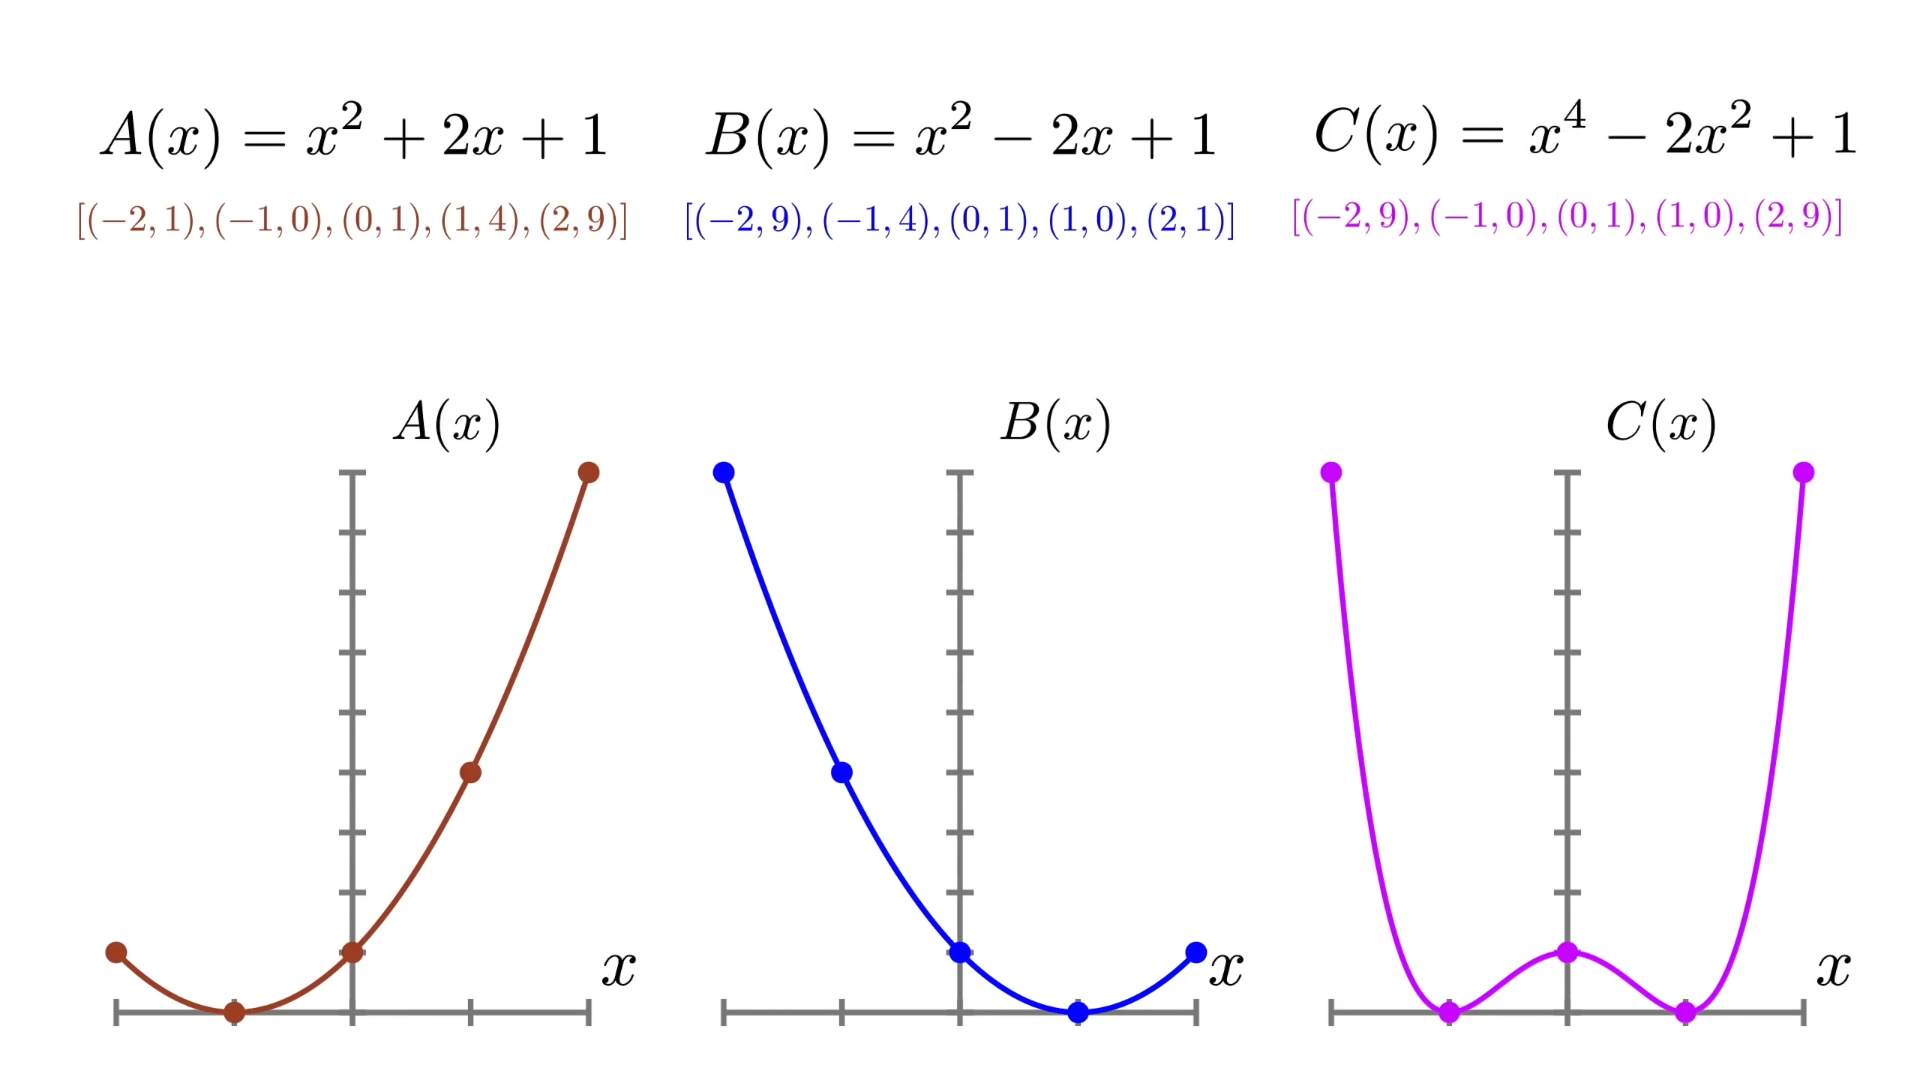
\includegraphics[width=0.8\textwidth]{beamer/images/interpolation.png}
    \end{figure}
\end{frame}

\begin{frame}{How can this be efficient?!}
    \begin{block}{}
        \begin{itemize}
            \uncover<1->{\item Sampling: evaluate the polynomial at $2n+1$ points, $\mathcal{O}(n^2)$}
            \uncover<2->{\item Pointwise multiplication: $\mathcal{O}(n)$}
            \uncover<3->{\item Interpolation: up to $\mathcal{O}(n^3)$}
        \end{itemize}
    \end{block}
    \begin{figure}
        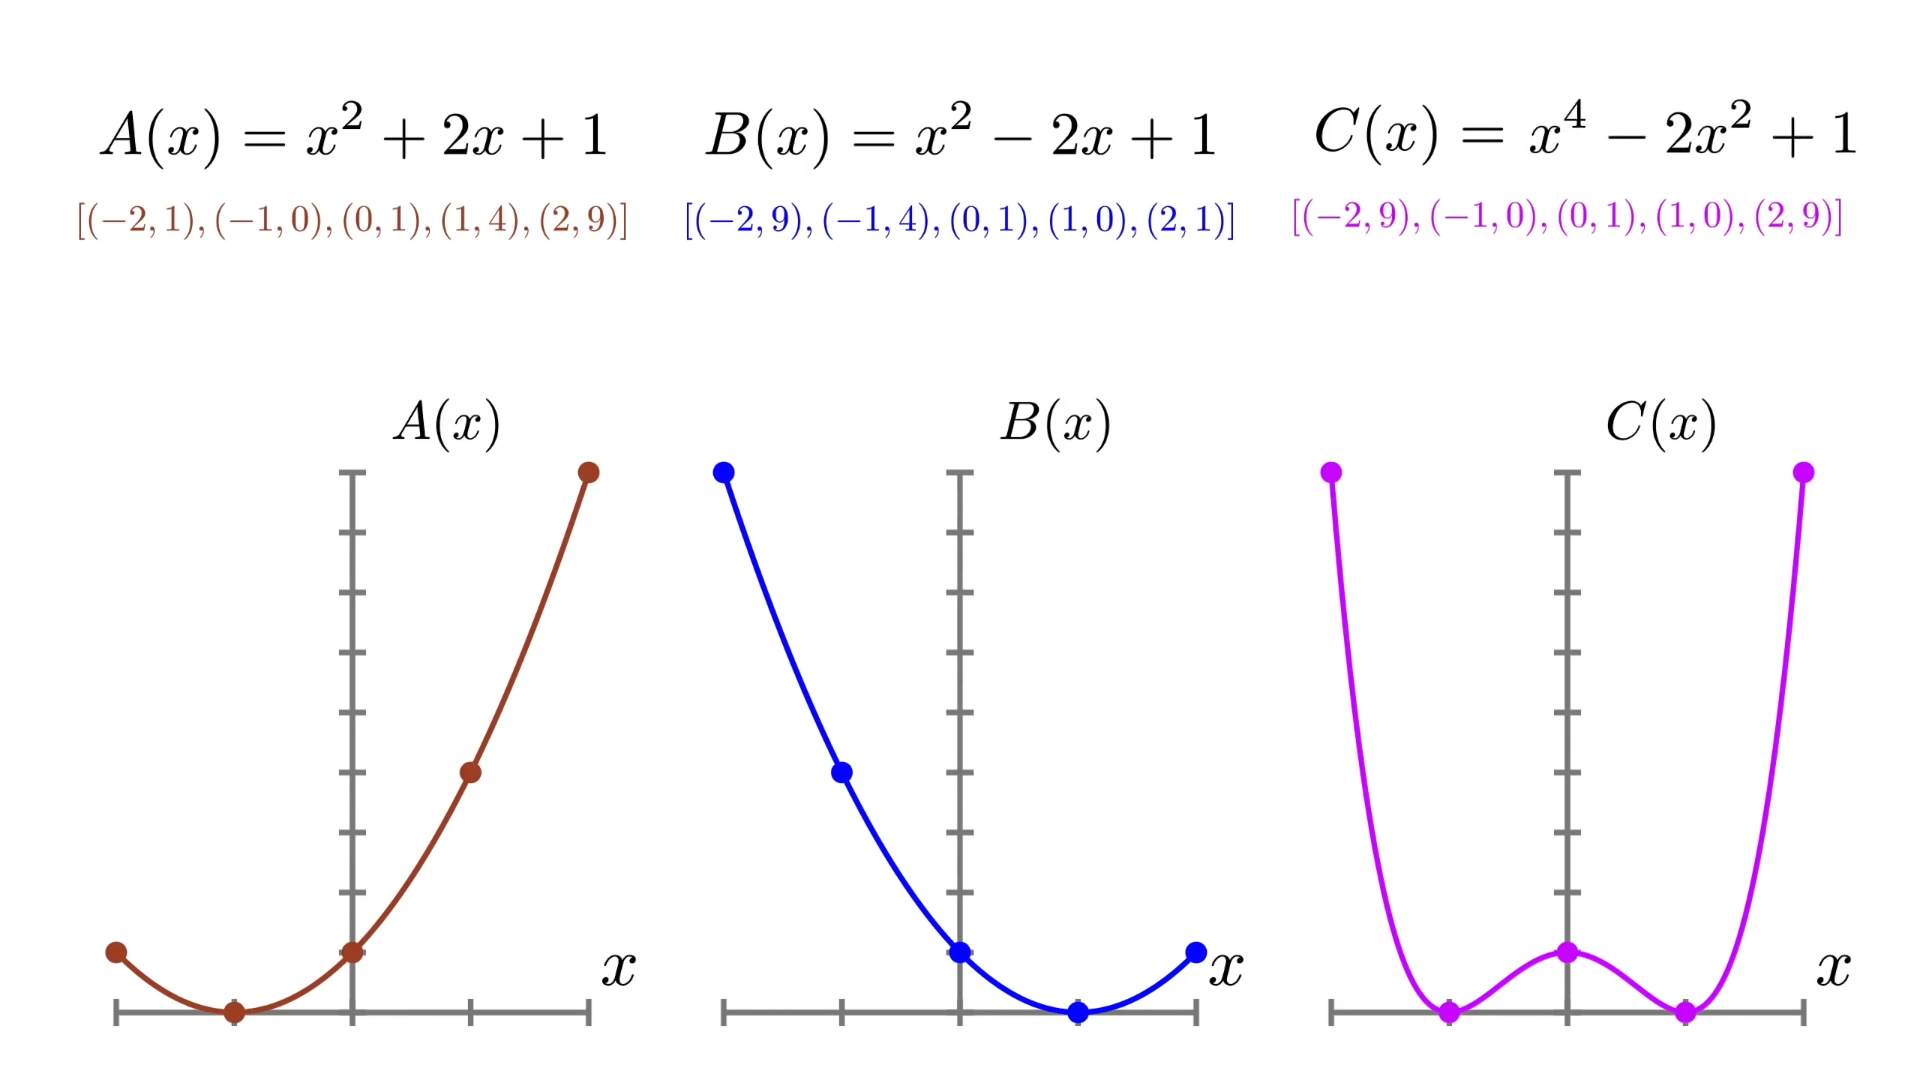
\includegraphics[width=0.8\textwidth]{beamer/images/interpolation.png}
    \end{figure}
\end{frame}

\begin{frame}{The Discrete Fourier Transform (in $\mathds{C}$)}
    \uncover<1->{
    \begin{block}{Sampling}
        Evaluate the polynomial at the $N$-th roots of unity $\rightarrow$ take the DFT
        \begin{equation*}
            \mathcal{F}(\omega_k) = \sum_{n=0}^{N} x_ne^{-\frac{2\pi i k}{N}n}
        \end{equation*}
    \end{block}
    }
    \uncover<2->{
    \begin{block}{Interpolation}
        Interpolate the points $\rightarrow$ take the inverse DFT
        \begin{equation*}
            \mathcal{F}^{-1}(X_k) = \frac{1}{N}\sum_{n=0}^{N} X_ne^{\frac{2\pi i k}{N}n}
        \end{equation*}
    \end{block}
    }
    \uncover<3->{
    Algorithms that calculate the DFT and its inverse are called Fast Fourier Transforms
    and can achieve $\mathcal{O}(n\log n)$ complexity.
    }
\end{frame}

\begin{frame}{FFT in finite fields}
    \begin{block}{}
        \begin{itemize}
            \item $a(x)$ and $b(x)$ are polynomials in $\mathds{F}_2[x]$
            \item Each coefficient $a_i, b_i \in \mathds{F}_2$ is a bit (0, 1)
        \end{itemize}
    \end{block}

    \begin{block}{}
        \uncover<2->{Problem: Finite fields (of characteristic 2) do not admit roots of unity\\}
        \uncover<3->{Solution: use powers of a primitive element\\}
        \uncover<4->{
        Caveat(s):
        \begin{itemize}
            \uncover<5->{\item The degree must be a power of 2: $n = 2^\ell$}
            \uncover<6->{\item Polynomials require a different representation}
        \end{itemize}
        }
    \end{block}
    \uncover<7->{
    \begin{block}{}
        Case study: the Lin-Chung-Han FFT~\cite{DBLP:conf/focs/LinCH14}
    \end{block}
    }
\end{frame}

\begin{frame}{Cantor basis}
    \begin{block}{Vector spaces and bases}
        $\mathds{F}_2^m$: vector space of $m$-bit strings over $\mathds{F}_2$, with $m$ power of 2\\
        Elements of $\mathds{F}_2^m$ are \emph{vectors}, linear combinations of the \emph{basis vectors}\\
        Basis vectors: $\mathbf{v} = (v_1, \cdots, v_m)$
    \end{block}
    \begin{block}{Canonical basis}
        \begin{equation*}
            \mathbf{v}=(1, \alpha, \alpha^2, \cdots, \alpha^{m-1})
        \end{equation*}
    \end{block}

    \begin{block}{Cantor basis}
        \begin{equation*}
            \mathbf{v} = (v_1, \cdots, v_m)
        \end{equation*}
        \begin{equation*}
            v_1 = 1 \qquad v_i^2+v_i = v_{i-1}
        \end{equation*}
    \end{block}
\end{frame}

\begin{frame}{Subspaces and vanishing polynomials}
    \begin{equation*}
        v_1 = 1 \qquad v_i^2+v_i = v_{i-1}
    \end{equation*}

    \begin{block}{Subspaces induced by Cantor basis}
        \begin{equation*}
            \mathbf{W}_0 := \{0\},\qquad \mathbf{W}_i := span\{v_0, \cdots, v_{i-1}\}
        \end{equation*}
        \vspace{5pt}
        with $\mathbf{W}_0 \subset \mathbf{W}_1 \subset \cdots \subset \mathbf{W}_m = \mathds{F}_2^m$ and $\dim(\mathbf{W}_i) = i$.
    \end{block}
    \uncover<2->{
    \begin{block}{Vanishing polynomials}
        \begin{equation*}
            s_i(x) = \prod_{a \in \mathbf{W}_i} (x-a)
        \end{equation*}
        \vspace{5pt}
        with $\deg(s_i(x)) = |\mathbf{W}_i| = 2^i$.
    \end{block}
    }
\end{frame}

\begin{frame}{Novelpoly basis}
    \begin{block}{Properties of the vanishing polynomials}
        \begin{itemize}
            \item linearity: $s_i(x) + s_i(y) = s_i(x+y)$
            \item recursivity: $s_{i+j}(x) = s_i(s_j(x))$, $s_i(v_{i+j}) = v_j$
            \item $s_i(v_i) = 1$ for $v_i$ element of the Cantor basis (\cite{DBLP:journals/corr/abs-1708-09746})
            \item all $v_i$ are roots of $s_{i+1}(x)$
        \end{itemize}
    \end{block}
    \uncover<2->{
    \begin{block}{Novelpoly basis}
        Cantor basis $\rightarrow$ Subspaces $\rightarrow$ Vanishing polynomials $\rightarrow$ Novelpoly basis
        \begin{equation*}
            X_k(x) = \prod (s_i(x))^{b_i}\qquad \text{with } k=\sum_{i=0}^{\log_2 n} b_i2^i
        \end{equation*}
        with $\deg(X_k(x)) = k$.
    \end{block}
    }
\end{frame}

\begin{frame}{Polynomial evaluation (sampling)} 
    \begin{block}{}
        We start from:
        \begin{itemize}
            \uncover<2->{\item $f(x) = g(X)$, a polynomial of degree $2^m$ in novelpoly basis}
            \uncover<3->{\item $\mathbf{W}_m = \mathds{F}_{2^m}$, the set of points to be evaluated}
        \end{itemize}
    \end{block}
    \uncover<4->{
    \begin{block}{}
        We want to get:
        \begin{itemize}
            \uncover<5->{\item $\{f(x) | x \in \mathbf{W}_m\}$, the evaluation of $f(x)$ at the points in $\mathbf{W}_m$}
        \end{itemize}
    \end{block}
    }
\end{frame}

\begin{frame}{The LCH FFT}
    \begin{block}{Divide et impera}
        Recursively split:
        \begin{itemize}
            \uncover<2->{\item The polynomial: $f_0(X) + f_1(X)X_{2^k}$}
            \uncover<3->{\item The set of points: $\mathbf{W}_{k-1}, (\mathbf{W}_{k} \setminus \mathbf{W}_{k-1})=\{w+v_{k-1} | w \in \mathbf{W}_{k-1}\}$}
        \end{itemize}
    \end{block}
    \uncover<4->{
    \begin{block}{Get 2 for the price of 1}
        Evaluate $f$ at $\mathbf{W}_{k-1}$; recall that:
        \uncover<5->{
        \begin{itemize}
            \item Elements in novelpoly basis are combinations of vanishing polynomials
            \item Vanishing polynomials are linear: $s_i(x) + s_i(y) = s_i(x+y)$
        \end{itemize}
        }
        \uncover<6->{
        Thus the evaluations at ($\mathbf{W}_k \setminus \mathbf{W}_{k-1}$) can be obtained starting from the evaluations at $\mathbf{W}_{k-1}$
        with a \emph{butterfly} unit
        }
    \end{block}
    }
\end{frame}

\begin{frame}{Butterfly unit}
    \begin{figure}[H]
    \begin{center}
        \begin{tikzpicture}
            \node (p0) at (0,3) {$p_0(X)$};
            \node (p1) at (0,0) {$p_1(X)$};
            \node (h0) at (10,3) {$h_0(X)$};
            \node (h1) at (10,0) {$h_1(X)$};
            \node (mul) at (3, 0) {$\bullet$};
            \node (add1) at (5, 3) {$\oplus$};
            \node (add2) at (7, 0) {$\oplus$};
            \node (sk) at (3.3, 1.5) {$s_k(\alpha)$};
            % arrow from p3 to p4
            \draw[->] (p0) to (add1);
            \draw[->] (p1) to (mul);
            \draw[->] (mul) to (add1);
            \draw[->] (mul) to (add2);
            \draw[->] (add1) to (add2);
            \draw[->] (add1) to (h0);
            \draw[->] (add2) to (h1);
        \end{tikzpicture}
    \end{center}
    \caption{Butterfly unit}
    \label{fig:butterfly} 
\end{figure}
\end{frame}

\begin{frame}{Frobenius map}
    \begin{block}{}
        We can use the Frobenius map
        \begin{equation*}
            \phi : \mathds{F}_2 \rightarrow \mathds{F}_2 \qquad x \mapsto x^2
        \end{equation*}
        to derive more values of a polynomial $f$ of degree $n$ from less evaluations.
    \end{block}
    \uncover<2->{
    \begin{block}{Frobenius partition}
        We can build a set of points $\mathbf{S} \subset \mathds{F}_{2^m}$ as:
        \begin{equation*}
            \mathbf{S} := v_{l+m/2}+\mathbf{W}_l = \{v_{l+m/2} + x \mid x \in \mathbf{W}_l\}
        \end{equation*}
        which has size $n^\prime = |\mathbf{S}| = |\mathbf{W}_l| = n/m$.
        \uncover<3->{
        By repeatedly applying $\phi$ to $\mathbf{S}$ we get
        \begin{equation*}
            \mathbf{S} \cup \phi(\mathbf{S}) \cup  \dots \cup \phi^{m-1}(\mathbf{S}) = \mathbf{O}
        \end{equation*}
        with $|\mathbf{O}| = n$.
        }
    \end{block}
    }    
\end{frame}

\subsection{Coding theory}

\begin{frame}{Error Correction Codes}
    \begin{figure}
        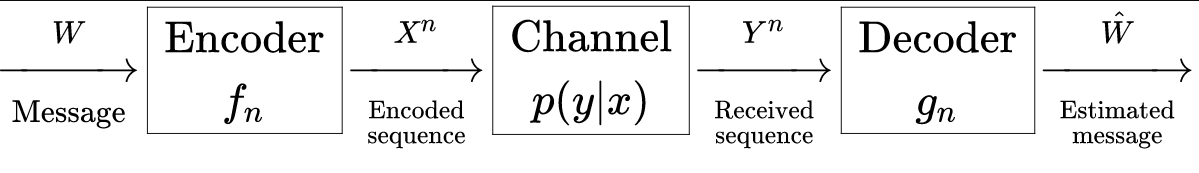
\includegraphics[scale=0.33]{beamer/images/ecc_channel.png}
        \end{figure}
    \begin{block}{}
        Problem: we want to send a message $m$ over a noisy channel.
        \begin{itemize}
            \uncover<2->{\item The channel is noisy: it introduces errors in the message}
            \uncover<3->{\item The receiver wants to recover the original message}
        \end{itemize}
    \uncover<4->{
    Solution: send, along with the message, information that allows the receiver to correct the errors.
    }
    \end{block}
\end{frame}

\begin{frame}{Linear codes}
    \begin{block}{}
        Let $\mathcal{V}$ be a vector space of dimension $n$ over $\mathds{F}_2$. A linear code $\mathcal{C} = [n,k]$ is 
        a subspace of $\mathcal{V}$ of dimension $k$.
        \uncover<2->{
        \begin{itemize}
            \item Messages are $k$ bits long
            \item We add $n-k$ bits to detect and correct errors (up to $\delta$)
        \end{itemize}
        }
    \end{block}
    \uncover<3->{
    \begin{block}{Generator Matrix}
        The matrix $\mathbf{G} \in \mathds{F}_2^{k\times n}$ is the generator matrix of $\mathcal{C}$ if
        \begin{equation*}
            \mathcal{C} = \{\mathbf{mG} \mid \mathbf{m} \in \mathds{F}_2^k\}
        \end{equation*}
    \end{block}
    }
\end{frame}

\begin{frame}{Syndrome}
    \begin{block}{Parity Check Matrix}
        The matrix $\mathbf{H} \in \mathds{F}_2^{(n-k)\times n}$ is the parity check matrix of $\mathcal{C}$ if
        \begin{equation*}
            \mathcal{C} = \{\mathbf{v} \in \mathds{F}_2^n \mid \mathbf{Hv}^\top = 0\}
        \end{equation*}
    \end{block}
    \uncover<2->{
    \begin{block}{}
        The syndrome of a word $\mathbf{v} \in \mathcal{C}$ is defined as:
        \begin{equation*}
            \mathbf{S}(\mathbf{v}) = \mathbf{Hv}^\top
        \end{equation*}
        \uncover<3->{This definition is equivalent to the one based on the generator matrix.}
    \end{block}
    }
\end{frame}

\begin{frame}{Syndrome Decoding}
    Given an encoded message, find the closest message w.r.t. a certain metric (\emph{i.e.} Hamming weight, \texttt{wt}()).
    \begin{block}{How hard can this be?}
        \begin{itemize}
        \uncover<2->{\item Take a word $\mathbf{x}$ with $\texttt{wt}(w)$}
        \uncover<3->{\item Calculate the syndrome $\mathbf{y}^\top = \mathbf{Hx}^\top$}
        \uncover<4->{\item Given $\mathbf{H}$ and $\mathbf{y}^\top$, retrieve $\mathbf{x}$}
        \end{itemize}
    \end{block}
    \vspace{10pt}
    \begin{center}
    \uncover<5->{This problem is \textbf{NP-complete}~\cite{DBLP:journals/tit/BerlekampMT78}.}
    \end{center}
\end{frame}

\subsection{Hamming Quasi-Cyclic}


\begin{frame}{Hamming Quasi-Cyclic}
    \begin{block}{}
        \begin{itemize}
            \item IND-CPA Public Key Encryption
            \item IND-CCA2 Key Encapsulation Mechanism
            \uncover<2->{\item Based on a variant of the syndrome decoding problem}
            \uncover<3->{\item Employs quasi-cyclic codes to shorten key sizes}
        \end{itemize}
    \end{block}
    \uncover<4->{
    \begin{block}{Codes}
        HQC employs two codes:
        \begin{itemize}
            \uncover<5->{\item a decodable $\mathcal{C} = [n, k]$ generated by $\mathbf{G}\in \mathds{F}_{2}^{k\times n}$ (public) }
            \uncover<6->{\item a random $[2n, n]$ code with parity-check matrix $\mathbf{H} = (\mathbf{I}_n | \mathbf{circ(h)})$}
        \end{itemize}
    \end{block}
    }
\end{frame}

\begin{frame}{Public Key Encryption}
    \begin{block}{Setup}
        Generate the parameters $(n, k, \delta, w, w_r, w_e)$ for the corresponding security level $\lambda$
    \end{block}
    \begin{block}{Key Generation}
        \begin{itemize}
            \uncover<2->{\item Generate $\mathbf{h} \xleftarrow{\$} \mathds{F}_2^n$ }
            \uncover<3->{\item Generate $(\mathbf{x, y}) \xleftarrow{\$} \mathds{F}_2^n$, with $\mathtt{wt}(\mathbf{x}) = \mathtt{wt}({\mathbf{y}}) = w$}
            \uncover<4->{\item Calculate $\mathbf{s = x + hy}$}
        \end{itemize}
        \uncover<5->{
        \begin{columns}
            \begin{column}{0.45\linewidth}
                \begin{center}
                    $\kpub = (\mathbf{h, s})$
                \end{center}
            \end{column}
            \begin{column}{0.45\linewidth}
                \begin{center}
                    $\kpri = (\mathbf{x, y})$
                \end{center}
            \end{column}
        \end{columns}
        }
    \end{block}
\end{frame}

\begin{frame}{Public Key Encryption}
    To encrypt a message $\mathbf{m} \in \mathds{F}_2^k$ :
    \begin{block}{Encryption}
        \begin{itemize}
            \uncover<2->{
            \item Generate $(\mathbf{r_1, r_2}) \xleftarrow{\$} \mathds{F}_2^n$, with $\mathtt{wt}(\mathbf{r_1}) = \mathtt{wt}({\mathbf{r_2}}) = w_r$
            \item Generate $\mathbf{e} \xleftarrow{\$} \mathds{F}_2^n$, with $\mathtt{wt}(\mathbf{e}) = w_e$
            }
            \uncover<3->{\item Calculate $\mathbf{u = r_1 + hr_2}$}
            \uncover<3->{\item Calculate $\mathbf{v = mG +sr_2 + e}$}
        \end{itemize}
        \uncover<4->{
        \begin{center}
            \textsf{ctx} = $(\mathbf{u, v})$
        \end{center}
        }
    \end{block}
\end{frame}

\begin{frame}{Public Key Encryption}
    \begin{block}{Decryption}
        From the \textsf{ctx} = $(\mathbf{u, v})$ and the private key \kpri = $(\mathbf{x, y})$:
        \begin{equation*}
            \uncover<2->{
            \begin{aligned}
                \mathbf{v - u\cdot y} & = \uncover<2>{ \mathbf{(mG +s\cdot r_2 + e) - (r_1 + h\cdot r_2)y = mG + x\cdot r_2 -r_1\cdot y + e}\\
                &\mathbf{ = mG + (x + h\cdot y)r_2 + e - (r_1\cdot y  + h\cdot r_2\cdot y)}\\
                &\mathbf{ = mG + x\cdot r_2 + h\cdot y\cdot r_2 + e - r_1\cdot y - h\cdot r_2\cdot y}\\}
                &\mathbf{ = mG + x_2 - r_1\cdot y + e}\\
            \end{aligned}
            }
        \end{equation*}
        \uncover<4->{
        So we have $\mathbf{m} = \mathcal{C}.\textsf{Decode}(\mathbf{v - u\cdot y})$ whenever
        \begin{equation*}
            \mathtt{wt}(\mathbf{x\cdot r_2 - r_1\cdot y + e}) \leq \delta
        \end{equation*}
        }
    \end{block}
\end{frame}

\begin{frame}{Side channel attacks}
    \begin{block}{}
        Devices running cryptosystems may expose secrets through \emph{side channels}
        Observable aspects of the system from which information can be extracted
    \end{block}
    \begin{figure}
        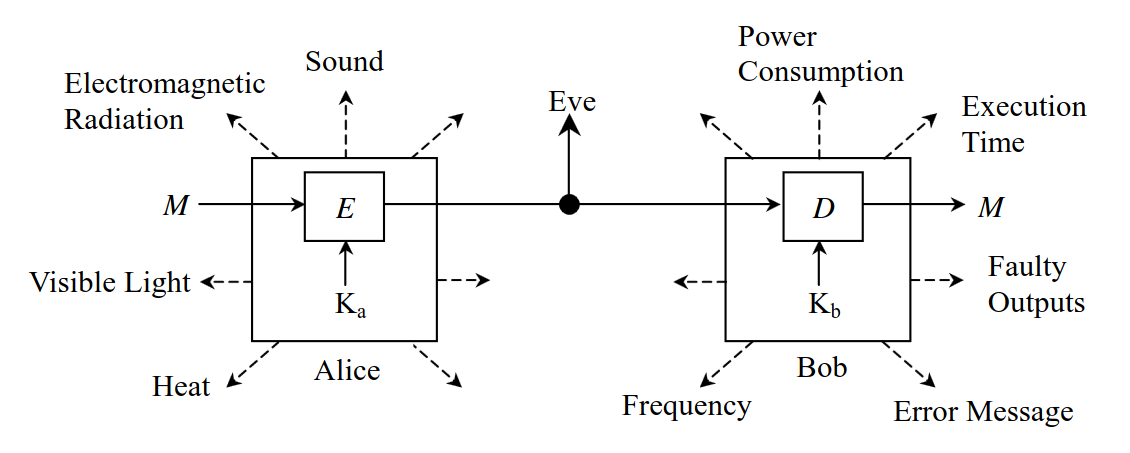
\includegraphics[width=0.8\textwidth]{beamer/images/sca.png}
    \end{figure}
\end{frame}

